% Chapter 3

\chapter{Chapitre 3 : Modélisation du problème de recherche de cibles} % Main chapter title

\label{Chapter3} % For referencing the chapter elsewhere, use \ref{Chapter1} 
%----------------------------------------------------------------------------------------
\section{Introduction}
L'étape de modélisation d'un algorithme basé intelligence en essaim est centrale, elle requiert une bonne analyse faite au préalable, ce qui est particulièrement nécessaire lorsqu’il s'agit des problèmes complexes.

Ce chapitre est dédié à la description de notre modélisation et conception; celles-ci regroupent la représentation de l'espace de recherche, de la solution, de la fonction objectif ainsi que tous les autres composants de l'environnement de recherche. 
Par la suite, nous passerons en revue des travaux connexes relatifs aux stratégies d’évitement d’obstacles, avant d’enchaîner avec la strategie choisie avec justification de ce choix. Enfin nous nous pencherons sur le principe de fonctionnement de l'algorithme génétique, qui sera utilisé comme outil de réglage de paramètres des méta-heuristiques de recherche de cibles.


\section{Modélisation de l'environnement de recherche}
\label{vuEnv}
Nous avons modélisé notre environnement de recherche par une représentation 2D dite \textit{"grid based"}, sous forme d’une matrice comme le montre la figure \ref{env}. Notre environnement est caractérisé par une surface préalablement fixée, afin que les bordures délimitent la zone de recherche. La forme de l’environnement est carrée telle que :
\begin{equation}
Surface = Taille_{Cot\acute{e}} * Taille_{Cot\acute{e}}.
\end{equation}

Taille$_{cot\text{é}}$ : C'est la longueur d'un segment du carré.

Dans cette grille, chaque case contient une valeur ainsi qu'une position / coordonnée  \textit{(x,y)}, composée d'une abscisse (\textit{x}) et d'une  ordonnée (\textit{y}). Plusieurs valeurs sont admissibles dans les cases, celles-ci permettent de distinguer les objets comme suit : 
\begin{itemize}
	
	\item[$\bullet$] \textbf{Cible :} Dans ce cas la valeur assignée à cette position est égale à \textbf{1}.
	\item[$\bullet$] \textbf{Portée d'une cible :} La valeur est bornée par \textbf{0} et \textbf{1}, ces derniers exclus.
	
	(valeur(x,y) $\in$ \textbf{] 0,1 [} )
	
	\item[$\bullet$] \textbf{Obstacle :} Sa valeur est égale à \textbf{-1}.
	\item[$\bullet$] \textbf{Zone neutre :} Prend la valeur \textbf{0}.\\
\end{itemize}

\begin{center}	  
	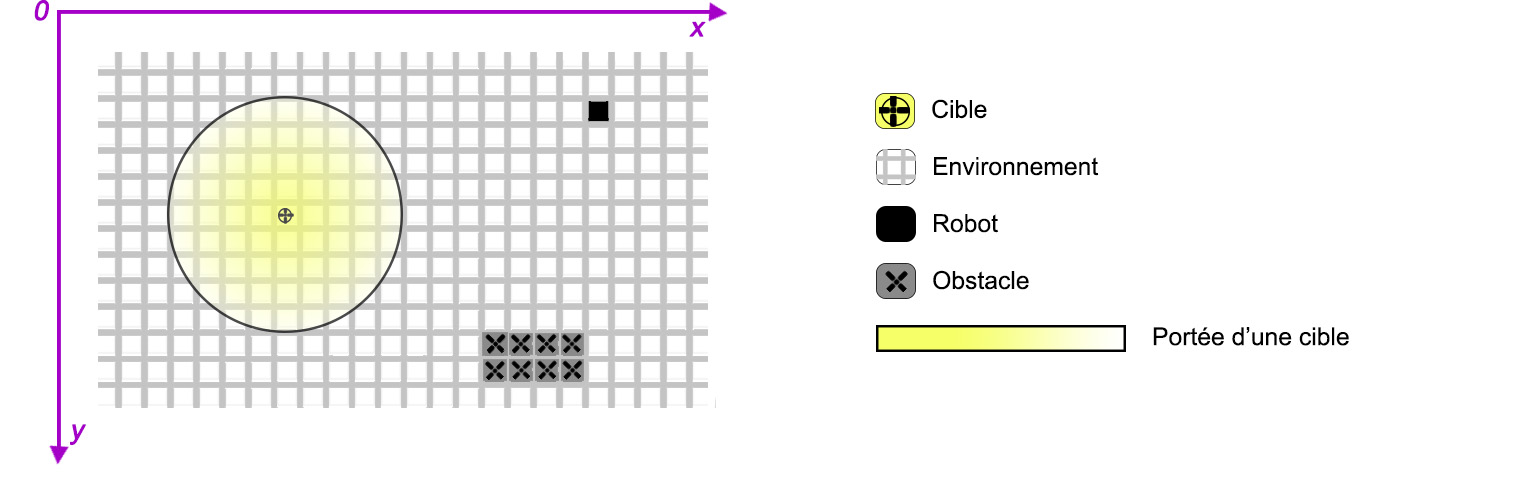
\includegraphics[width=1\textwidth]{env.jpg}%
	\vspace{-0.1 cm}
	\captionof{figure}{Représentation de l'environnement.}\label{env}%
\end{center}








\subsection{Représentation de la solution}
\label{sol}
Le but étant de trouver les cibles dans un environnement inconnu; l'espace des solutions à explorer n'est autre que notre environnement 2D composé de positions que nous appellerons aussi "solutions". 

Une solution optimale est une position géographique de coordonnée \textit{(x,y)}, elle est décrite par la valeur de sa case. La figure \ref{solution} représente une solution dans l'environnement de recherche. 

Dans le cas de multiples cibles on devra trouver autant de solutions optimales que de cibles, telles que chaque solution correspond à une case de valeur 1.
\begin{center}	  
	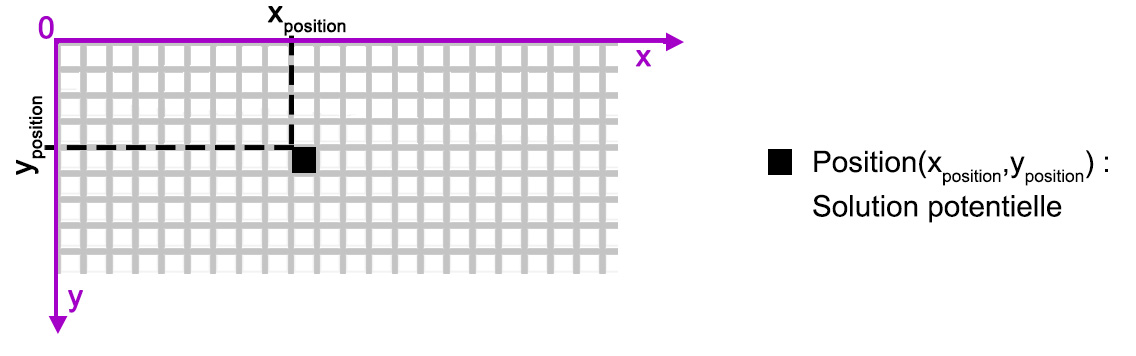
\includegraphics[width=0.8\textwidth]{Solution.jpg}%
	\vspace{-0.1 cm}
	\captionof{figure}{Représentation d'une solution dans notre modélisation.}\label{solution}%
\end{center}

Une solution doit satisfaire deux contraintes. D'abord, celle de la bornitude par les dimensions de l'environnement de recherche, ce dernier étant carré de taille $Taille_{Cot\acute{e}}$,
une solution est telle que:
\begin{equation}
\left\lbrace
\begin{array}{ccc}
0 \leq Position.x < Taille_{Cot\acute{e}}\\
0 \leq Position.y < Taille_{Cot\acute{e}}
\end{array}\right.
\end{equation}
Puis en tenant compte qu'une position contenant un obstacle n'est pas une solution admissible, soit :
\begin{equation}
environnement.get(Position.x , Position.y) \neq -1
\end{equation}



\subsection{Fonction objectif \label{fitness}}
Les solutions ont besoin d'être évaluées pour mesurer leurs distances par rapport à une cible. Ainsi, on pourra choisir la plus proche à chaque itération.

Notre fonction objectif varie selon l'intervalle borné suivant : [0,1]. Elle est égale à la valeur captée par les capteurs du robot, telle que plus la valeur se rapproche du 1, plus le robot est proche de la cible, car son émission est plus importante. Comme nous le verrons plus bas (Section \ref{porteee}), l'évaluation se fait sur les cases visibles par le robot, cela à travers son champ de vision (comportant un certain nombre de cases).

\subsection{Les cibles}
Une cible occupe une case unique ayant une valeur de 1, elle possède aussi une portée circulaire fixe, relative à l'émission de signaux perceptibles par les robots.\\ 

Comme on peut le voir dans la figure \ref{cible}, la portée décroît à partir de la position de la cible valant "1", jusqu'à la valeur "0" lorsque la distance par rapport à la cible excède la taille de la portée. Autrement dit, les valeurs représentatives des émissions de la cible sont inversement proportionnelles à la distance des positions incluses dans la portée.

\begin{center}	  
	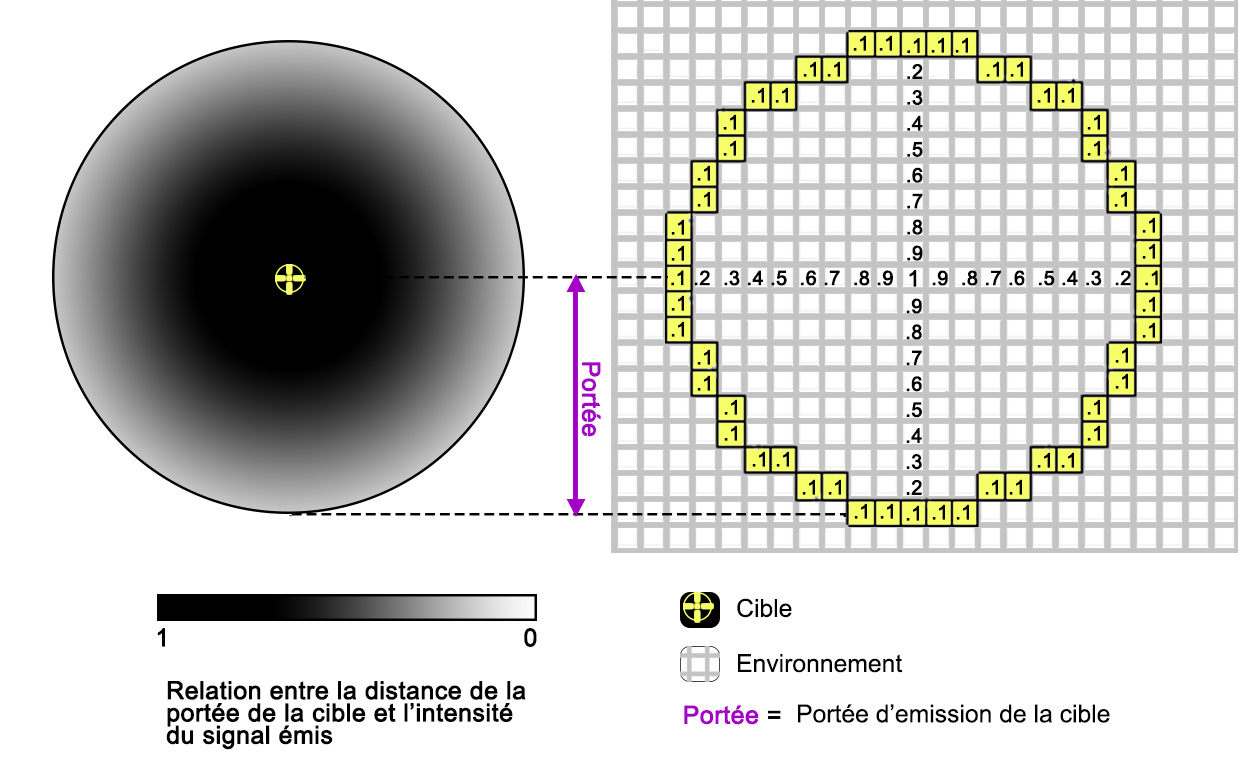
\includegraphics[width=0.8\textwidth]{cible.jpg}%
	\vspace{-0.1 cm}
	\captionof{figure}{Représentation de la portée d'une cible dans notre modélisation.}\label{cible}%
\end{center}

\paragraph{Remarque:}
Une fois qu'une cible est atteinte par un robot, elle est désactivée, elle arrête alors d'émettre des signaux. Nous avons modélisé cette action par la mise à zéro des cases de la matrice de l'environnement constituant la portée de cette cible.


\subsection{Les obstacles}
Un obstacle est considéré comme un objet fixe (statique) occupant une certaine surface de l'environnement et empêchant les robots de s'y positionner ou de la traverser.

Les environnements peuvent être catégorisés en trois (3) types selon la densité des obstacles, soient:

\begin{itemize}
	\item[$\bullet$] \textbf{Environnements simples (sans obstacles) :} Ceux-là ne contiennent que la ou les cible(s).
	\item[$\bullet$] \textbf{Environnements avec obstacles :} Comportant un nombre réduit d'obstacle de forme rectangulaire ainsi que la ou les cible(s).
	
	La taille d'un obstacle est comprise entre 2\% et 4\% de la taille de l'environnement. Quant au nombre d'obstacles, il appartient à l'intervalle [15 , 25] obstacles.
	
	\item[$\bullet$] \textbf{Environnements complexes :} Ils possèdent plus d'obstacles qui sont plus grands en termes de superficie que ceux de la catégorie précédente, en plus de la ou les cible(s).\\
	Dans ces environnements, la taille d'un obstacle est comprise entre 4\% et 6\% de la taille de l'environnement avec une densité de [25 , 35] obstacles.
\end{itemize}
\textbf{ }

Face aux différents types d'environnement existants, le choix d'une bonne stratégie d'évitement d'obstacles adaptée à notre modélisation devient crucial.


\section{Stratégies d'évitement d'obstacles}
Une stratégie d'évitement d'obstacles est nécessaire pour la navigation des robots dans des environnements à obstacles et complexes.
Le but des méthodes d'évitement d'obstacles est de trouver une trajectoire sûre (sans obstacles) entre deux positions, c’est-à-dire entre la position initiale d’un robot et sa position destination ou but.


\subsection{Description des approches existantes}
Les techniques les plus utilisées pour l'évitement d'obstacles sont décrites ci-dessous:

\subsubsection{Les algorithmes Bug  \cite{Sara,Bug}}
Les algorithmes Bug1 et Bug2 sont des méthodes anciennes et simples. Ils réduisent le robot en un point dans un plan 2D détectant les obstacles via capteurs tactiles. Ils sont basés sur deux comportements : \textit{"déplacement vers le but"} et \textit{"suivi d’une limite"}. 

\paragraph{Bug1 :}Tant que le robot n’a pas rencontré d’obstacle, il suit le comportement \textit{"déplacement vers le but"}, il se dirige tout droit vers la position but ($T$), lorsqu’il rencontre un obstacle en un point ($H_{i}$) il bascule vers le comportement \textit{"suivi d’une limite"} en faisant un tour complet sur l’obstacle. À partir de là il détermine le point du périmètre de l’obstacle  ($L_{i}$) le plus proche de la position but et s’y positionne. Ce processus se réitère jusqu’à atteindre la destination. (voir la figure \ref{bug}).

\paragraph{Bug2 :}
 Il exploite la première solution prometteuse qu’il trouve. Durant le comportement \textit{"déplacement vers le but"}, le robot se déplace selon des lignes droites reliant la position initiale ($S$) du robot et la position but ($T$). Quand un obstacle est rencontré, le robot adopte le comportement \textit{"suivi d’une limite"}, consistant à faire le tour de l’obstacle, jusqu’à atteindre un nouveau point  ($H_{i}$) qui appartient à la droite ($S$ , $T$) (voir la figure \ref{bug}).
Le processus est répété tant que la position but n’est pas atteinte par le robot.

\begin{center}	  
	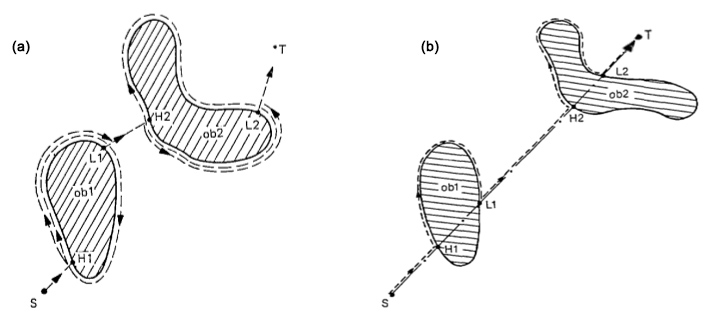
\includegraphics[width=0.75\textwidth]{../Figures/Bug.jpg}%
	\vspace{-0.1 cm}
	\captionof{figure}{Calcul du chemin du robot par les algorithmes Bug : (a) Bug1, (b) Bug2 \cite{Bug}. }\label{bug}%
\end{center}

\subsubsection{La méthode basée sur les champs de potentiel PF (Potential Field) \cite{Sara}}
Cette méthode a été proposée pour la première fois par Oussama Khatib \cite{Khatib}. Elle considère le robot comme une particule plongée dans un champ de potentiel, celui-ci régie par deux forces, soient : 

Force attractive $U_{attract}$: générée par le but.

Force répulsive $U_{r\acute{e}puls}$: générée par les obstacles.\\

Le robot calcule d’une manière itérative son prochain mouvement, suivant une direction résultante des sommes de différents champs potentiels (voir la figure \ref{pf}). La direction est donnée par la fonction :
 
\begin{equation}
F = - \bigtriangledown (U_{attract} + U_{r\acute{e}puls})
\end{equation}


\begin{center}	  
	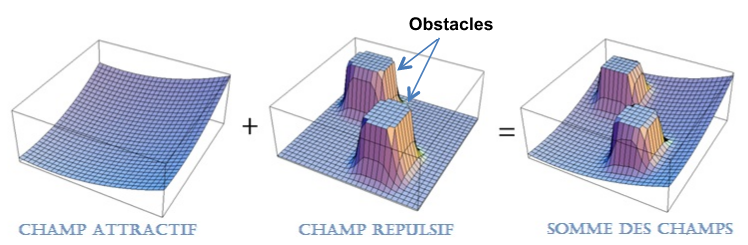
\includegraphics[width=0.75\textwidth]{../Figures/FP.png}%
	\vspace{-0.1 cm}
	\captionof{figure}{Champs de potentiel pour un environnement contenant deux obstacles et une position but.\cite{ImagePF}}\label{pf}%
\end{center}
	
\subsubsection{La méthode basée sur la fenêtre dynamique DW (Dynamic Window) \cite{Sara}}
La fenêtre dynamique est une méthode proposée par \textit{Burgardand} et \textit{Thruncite} \cite{window}. Elle vise à choisir un couple \textit{(v,w)} représentant respectivement la vitesse linéaire et angulaire du robot, permettant d’éviter les obstacles perçus localement. Sur la base des différents couples possibles, DW opte pour le couple de vitesses le plus pertinent. Comme le montre la figure \ref{dw}, la zone de recherche est limitée par une fenêtre dynamique basée sur les limitations dynamiques du robot et les vitesses admissibles et atteignables durant un laps de temps donné.
\begin{center}	  
	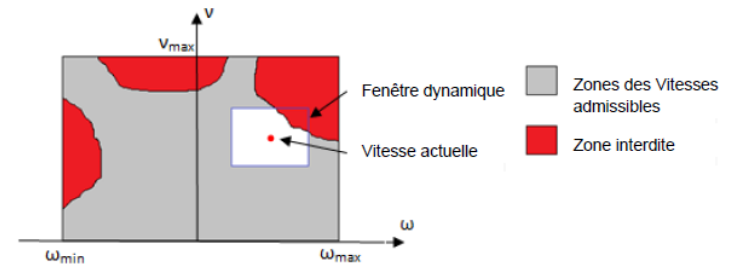
\includegraphics[width=0.75\textwidth]{../Figures/DW.png}%
	\vspace{-0.1 cm}
	\captionof{figure}{L'approche de la fenêtre dynamique montrant les régions admissibles et interdites par rapport à la fenêtre dynamique des vitesses atteignables par le robot \cite{Sara}.}\label{dw}%
\end{center}
		
\subsubsection{La logique floue}
La logique floue est une branche de l’intelligence artificielle et des mathématiques qui a été appliquée à des problèmes de commandes (Bühler 1997) \cite{FuzzyLogic}. Cette technique se base sur la déduction de deux commandes : la vitesse linéaire et angulaire selon les variables floues des données en entrées, qui sont : la vitesse (\textit{v}) du robot et l’angle ($\alpha$) entre le robot et l’obstacle, en plus d’une base de règles afin d’éviter les obstacles \cite{Cai2013}.
		
		
\subsubsection{L'échantillonnage de l'espace d'entrée ISS (Input Space Sample) }
À partir d'un état initial du robot, le modèle prédictif du système est utilisé pour la génération d'un ensemble de trajectoires. Celles-ci peuvent être triées selon une fonction de coût. L'exemple d'un ensemble de trajectoires générées en utilisant la technique par échantillonnage de l'espace d'entrées est illustré dans la figure \ref{ech}.

Selon les obstacles visibles par le robot, certaines trajectoires seront bannies de l'ensemble des trajectoires admissibles \cite{Sara}, comme il est le cas de \textit{S1, S2, S7, S8} et \textit{S9}.
		
Les travaux de \textit{Kelly} et \textit{Stentz} \cite{echantillonnage} font partie des premiers travaux basés sur cette technique.
		
\begin{center}	  
	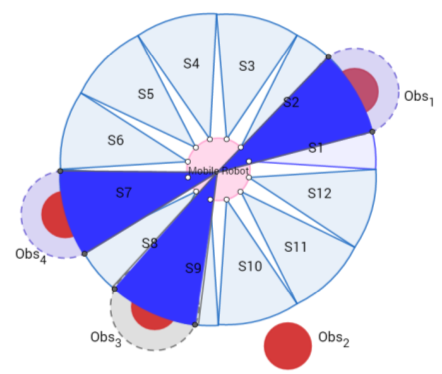
\includegraphics[width=0.5\textwidth]{../Figures/echan.png}%
	\vspace{-0.1 cm}
	\captionof{figure}{Ensemble de trajectoires
	générées par échantillonnage de l'espace d'entrées \cite{imageEch}.}\label{ech}%
\end{center}


\subsection{Discussion et choix}
Les algorithmes bug1 et bug2 sont faciles à mettre en œuvre et peu gourmands en termes de  mémoires. Cependant, ils nécessitent des déplacements supplémentaires et souvent la trajectoire trouvée est loin d'être optimale (trajectoires comportant trop de détours supplémentaires augmentant ainsi la distance pour atteindre la position but).\\ 

Les méthodes de champ de potentiel et de logique floue, sont facilement adaptables aux formules des méta-heuristiques disposant d’une vélocité telles qu'ESWSA. En revanche, elles sont difficiles à mettre en pratique pour d'autres méthodes dont BSO et EHO, car le calcul des positions est indépendant de la direction de l’ancienne position vers la nouvelle.

De plus, elles ne permettent pas de détecter un passage entre des obstacles assez proches. Encore pire, le robot risque de ne jamais atteindre la position but, si ce dernier est à proximité directe d'un obstacle.\\  

D'autre part, la méthode de la fenêtre dynamique (DW) n'est pas sujette aux limites précédemment citées. Mais elle peut être vu comme une recherche exhaustive d'une trajectoire optimale selon la dimension de la fenêtre, car pour une fenêtre de taille (\textit{x, y}) nous aurons \textit{x * y} paires (\textit{v, w}) à tester.\\

Enfin, la stratégie d'échantillonnage, n'est pas concernée par les problèmes cités ci-dessus dans le cadre de notre modélisation. Elle est simple et efficace, mais son plus grand avantage est qu'elle peut être directement adaptée ou intégrée dans d'autres concepts ou algorithmes.\\

Suite à l'analyse faite ci-dessous des avantages et inconvénients de chaque approche par rapport à notre modélisation, notre choix s'est porté sur la stratégie d'\textbf{échantillonnage} qu'on a jugé comme étant la plus adéquate.


\subsection{Paramètres de la méthode d'échantillonnage}
L'échantillonnage de l'espace local des robots est régi par plusieurs paramètres devant être fixés au préalable, soient : 

\subsubsection{Champ de vision}
L'espace local d'un robot est divisé en quatre zones de 90$\textordmasculine$, comme le montre la figure \ref{zones} : $"$NE: Nord-Est, NW: Nord-Ouest, SW: Sud-Ouest, SE: Sud-Est$"$.

Le champ de vision d'un robot est d'un angle de 90$\textordmasculine$, choisi selon la zone contenant la droite reliant la position du robot à la position but.\\

Afin de déterminer la zone concernée, nous devons effectuer deux opérations de soustraction sur les coordonnées du robot ($x_{R}$,$y_{R}$) et celles de la position destination ($x_{but}$,$y_{but}$).
Les zones relatives aux résultats de ces opérations sont représentées dans le schéma ci-dessous. 
\begin{center}	  
	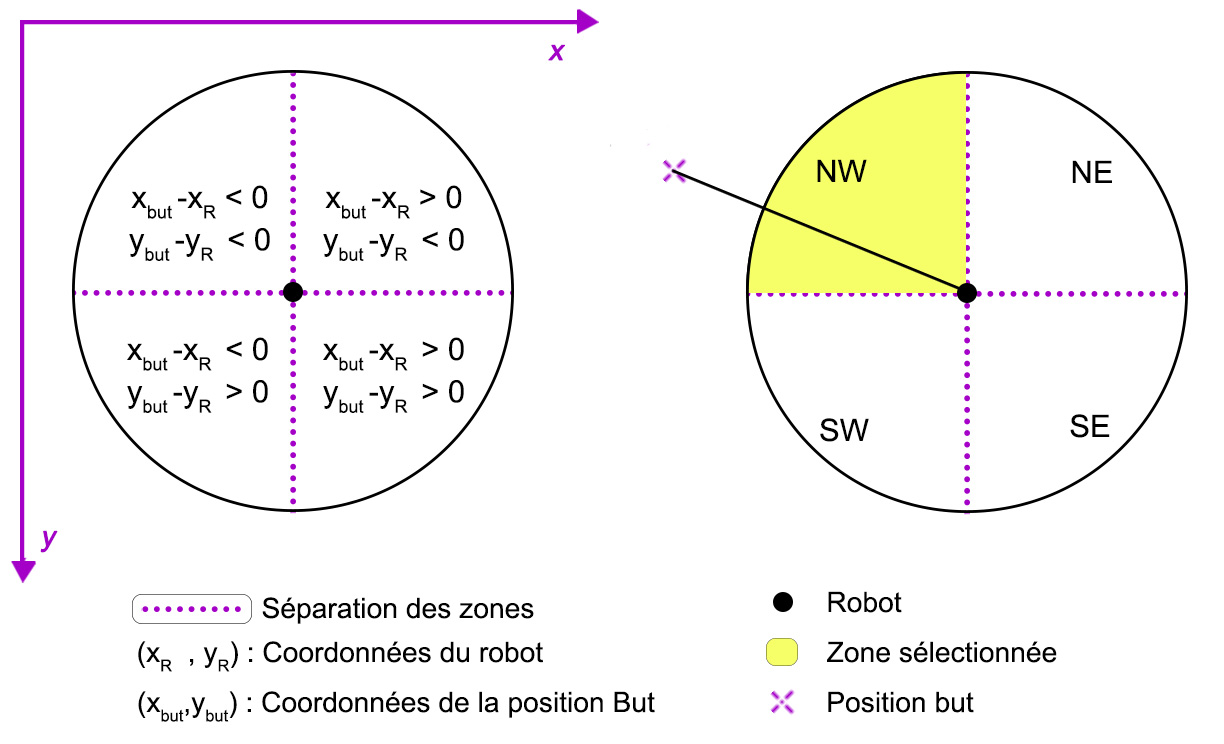
\includegraphics[width=0.7\textwidth]{Angle_de_vue.jpg}%
	\vspace{-0.1 cm}
	\captionof{figure}{Détermination de l'angle de vue d'un robot dans notre modélisation.}\label{zones}%
\end{center}

\subsubsection{Portée locale d'un robot}
\label{porteee}
Chaque robot possède une portée locale, celle-ci forme une surface circulaire dont le robot est le centre. Le rayon de ce cercle est limité par la portée des capteurs présents sur le robot.

Dans notre modélisation, cette portée locale est fixée à une distance de dix positions du robot. La zone maximale visible par chacun de nos robots est représentée dans la figure \ref{portee} qui suit:


\begin{center}	  
	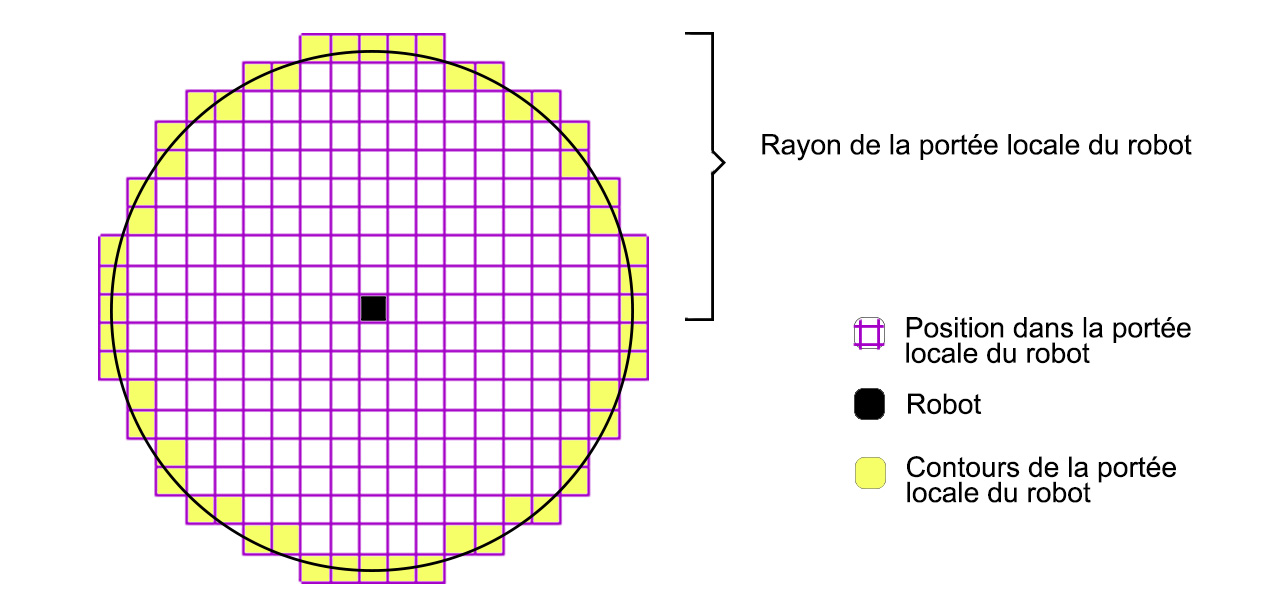
\includegraphics[width=0.69\textwidth]{portee.jpg}%
	\vspace{-0.1 cm}
	\captionof{figure}{Représentation de la portée locale d'un robot dans notre modélisation.}\label{portee}%
\end{center}

Il est à noter que les robots ont cette portée de vue durant tout le parcours fait, c'est-à-dire que tout le long de leurs déplacements, une vérification de cette surface accessible est effectuée. 

Nos robots prennent place dans les meilleures positions visibles dans leurs portées, cela à travers le processus suivant :\\

\begin{algorithm}[H]
	\SetAlgoLined
	\KwIn{$P$ : position du robot,\\
		\hspace{1.3cm}$portee$ : Portée des capteurs = 10,\\
		\hspace{1.3cm}$env$ : Matrice de dimension M*M}
	
	\KwResult{meilleurePosition : Meilleure position maximisant la fonction objectif}
	
	\vspace{0.2cm}
	
	%\tcc{Initialisation}
	$meilleureLocale \gets env.valeur( P_x , P_y)$\;
	$meilleurePosition \gets Position(P_x,P_y)$\;
	
	\vspace{0.2cm}
	
	%	\tcc{Evaluation}
	\For{i $\gets$ -portee \KwTo +portee}{
		\For{j $\gets$ -portee \KwTo +portee}
		{  
			\vspace{0.2cm}
			
			%\tcc{Vérification si la position est valide (bornée par les dimensions de l'environnement) et est dans le rayon accessible}
			
			\If{$env.valide( P_x + i, P_y + j ) $ \textbf{And}  $ i^2 + j^2 \leq portee^2$} {
				$b \gets env.valeur (  P_x + i, P_y + j)$\;
				\If{$meilleureLocale < b$ }{
					$	meilleureLocale \gets b $\;
					$meilleurePosition \gets Position( P_x + i, P_y + j)$\;
				}
			}
		}
	}
	
	\Return$meilleurePosition$\;
	
	\caption{Meilleure position dans la portée du robot}
\end{algorithm}



\subsubsection{Trajectoire}
Une trajectoire est modélisée par une droite reliant deux positions successives, cette droite est un ensemble de cases extraites selon l'équation de la droite, \textit{Bresenham} \cite{line} l'a exploité pour en déduire l'algorithme \ref{codeLine} suivant : 




\noindent
\begin{minipage}[t]{0.45\textwidth}
	\vspace{-0.5cm}
	\begin{algorithm}[H]
		
		\SetAlgoLined
		\DontPrintSemicolon
		\KwIn{$x_0$,$y_0$,$x_1$,$y_1$ }
		%\KwOut{}
		
		\SetKwData{dx}{dx}
		\SetKwData{dy}{dy}
		\SetKwData{sx}{sx}
		\SetKwData{sy}{sy}
		\SetKwData{x}{$x_{0}$}
		\SetKwData{y}{$y_0$}
		\SetKwData{xx}{$x_{1}$}
		\SetKwData{yy}{$y_1$}
		\SetKwData{err}{err}
		\SetKwData{e}{e2}
		
		\SetKwFunction{Abs}{Abs}
		\SetKwFunction{setPoint}{setPoint}
		
		\dx = \Abs(\xx-\x);
		\dy = -\Abs(\yy-\y);
		
		\lIf{\x<\xx}{\sx = 1;}\lElse{\sx = -1;}
		\lIf{\y<\yy}{\sy = 1;}\lElse{\sy = -1;}
		
		\err = \dx+\dy;
		
		\While{True}{
			\setPoint(\x,\y);
			
			\e = 2*\err;
			
			\lIf{\e >= \dy} {
				\lIf{\x == \xx}{ break;}
				\err += \dy; \x += \sx;
			}
			\lIf{\e >= \dx} {
				\lIf{\y == \yy}{ break;}
				\err += \dx; \y += \sy;
			}
		}
		\caption{line-drawing algorithm \cite{line}}
		\label{codeLine}
	\end{algorithm}
\end{minipage}\hfill
\begin{minipage}[t]{0.45\textwidth}
	%\vspace{0.1cm}
	\centering\raisebox{\dimexpr \topskip-\height}{%
		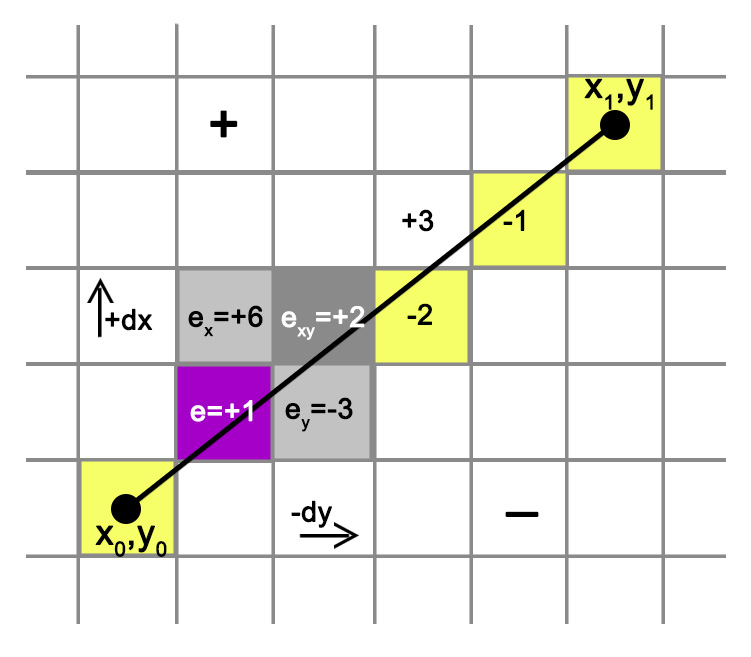
\includegraphics[width=1\textwidth]{line.jpg}}
	\captionsetup{width=0.7\linewidth}
	\captionof{figure}{Sélection des points (cases) d'une droite avec l'algorithme de BRESENHAM.}
	\label{line}
\end{minipage}

\vspace{0.5cm}
Grâce à cet algorithme de Bresenham, nous pouvons au lieu de chercher à dessiner la droite à partir de deux positions, comme le montre la figure \ref{line}, l'exploiter pour vérifier si une trajectoire comporte des obstacles ou non.




\subsubsection{Critères de choix de la trajectoire}
Une fois que nous sommes en mesure de déterminer si une trajectoire est admissible (sans obstacles) ou interdite (contient des obstacles), vient l'étape de sélection de la trajectoire admissible la plus adéquate.

Cette seconde étape revient à choisir la meilleure trajectoire parmi celles admissibles, en minimisant la distance entre la position choisie (accessible) et la position destination de notre robot.
Les deux étapes sont illustrées dans la figure \ref{choix} ci-dessous :

\begin{center}	  
	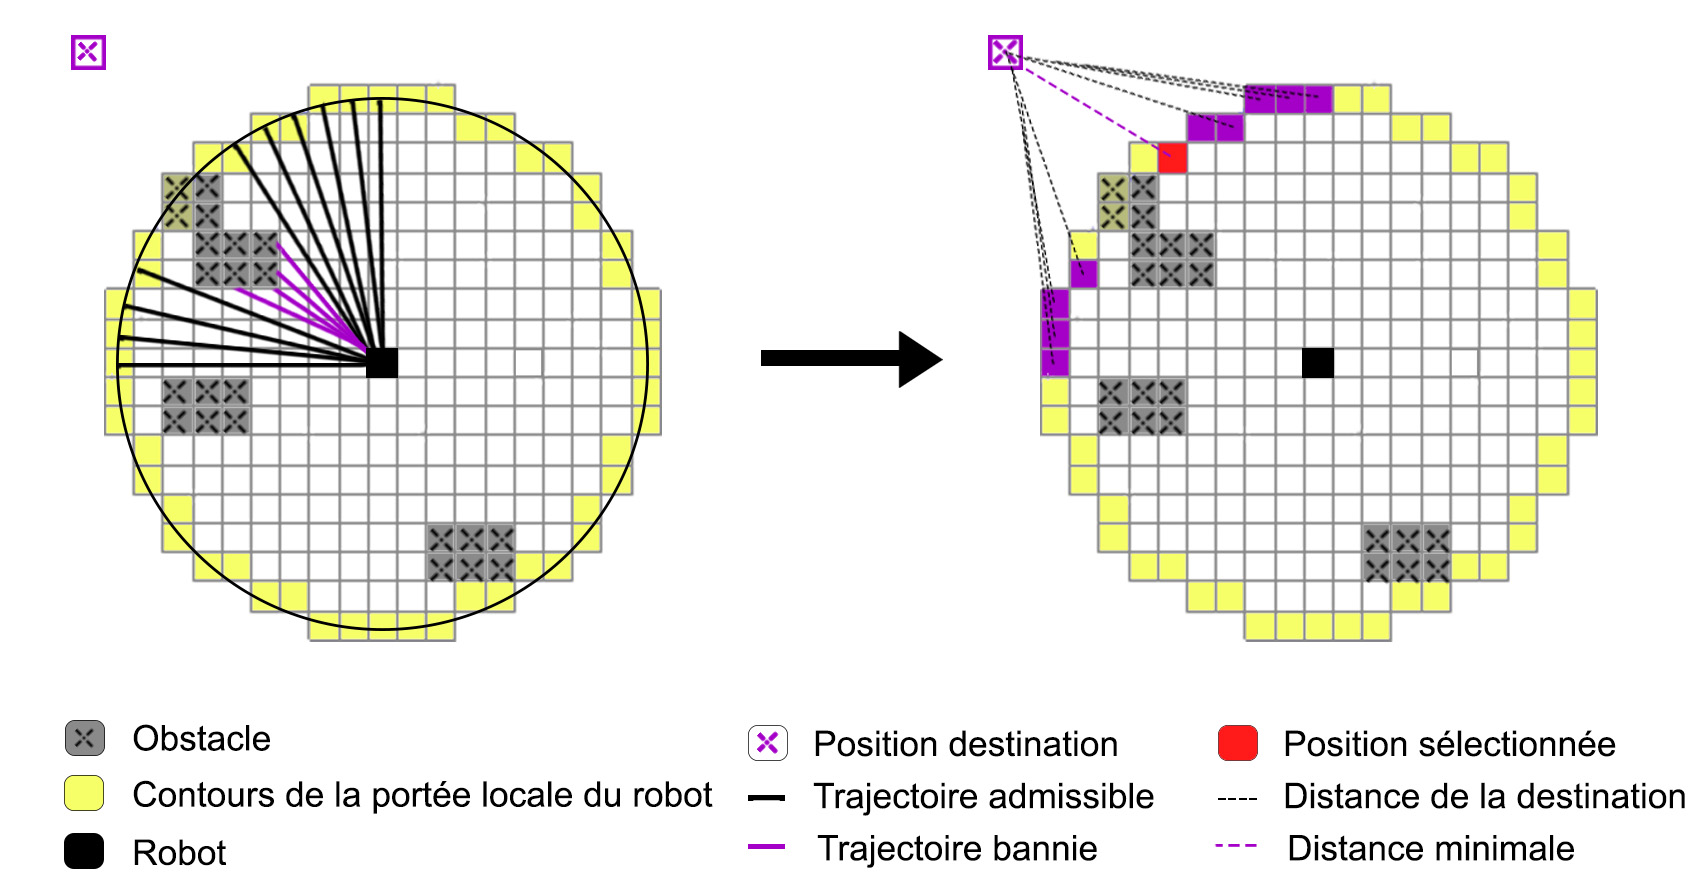
\includegraphics[width=0.9\textwidth]{choix.jpg}%
	\vspace{-0.1 cm}
	\captionof{figure}{Choix de la trajectoire à suivre par le robot dans un environnement à obstacle.}\label{choix}%
\end{center}

\paragraph{Remarque:} Si la position de destination est à une distance inférieure à la portée du robot (inférieure à dix cases.), le même procédé est effectué avec une portée égale à la distance entre le robot et la position destination.

\paragraph{Autres cas de figure}

Plusieurs cas de figure existent selon la position des obstacles par rapport à celle du robot, pour cela nous avons étudié toutes les possibilités pour garantir le bon fonctionnement de notre approche dans tous les environnements.\\

La figure \ref{choix_annexe} représente deux cas de figure se produisant souvent dans des environnements complexes.
Lorsque aucune trajectoire admissible n'est trouvée dans le champ de vision initial du robot (90$\textordmasculine$), on l'élargit aux zones adjacentes de 90$\textordmasculine$ allant ainsi à un champ de vision qui équivaut à 270 $\textordmasculine$. Ceci simulera une rotation du robot sur lui-même (voir schéma de droite).

Si le robot ne trouve toujours pas de trajectoire admissible, une nouvelle position destination est demandée.\\

Dans le cas où la position destination est alignée sur un des deux axes avec la position actuelle du robot (c'est-à-dire qu'ils possèdent la même abscisse ou même ordonnée), notre robot aura une vue sur les 180$\textordmasculine$ dont la droite (position du robot - position destination) est commune (schéma de gauche).
\noindent
\begin{center}	  
	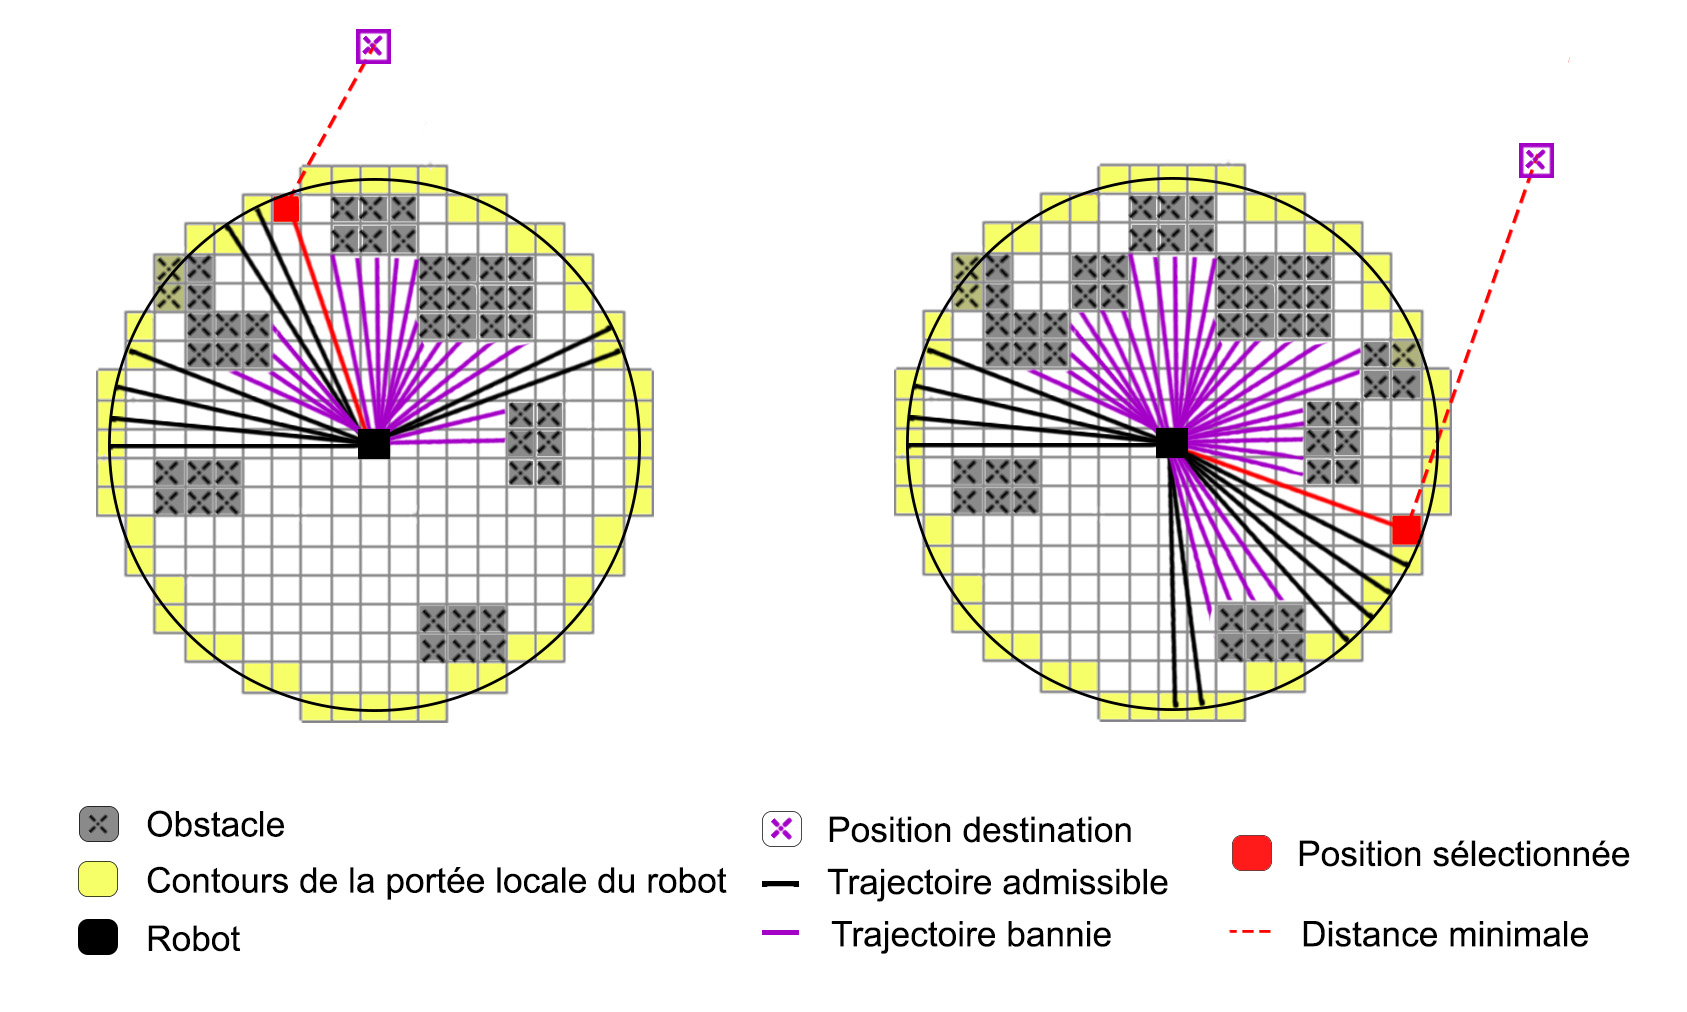
\includegraphics[width=0.9\textwidth]{choix_annexe.jpg}%
	\vspace{-0.1 cm}
	\captionof{figure}{Choix de la trajectoire à suivre par le robot dans des situations complexes.}\label{choix_annexe}%
\end{center}


\section{Auto-Paramétrage avec GA}
\label{génétique}
\subsection{Modélisation}
\subsubsection{Solution}
Une solution pour notre algorithme génétique est un paramétrage pour une de nos approches de résolution. Elle est représentée par un vecteur de paramètres.\\
Vu que nos méta-heuristiques n'ont ni le même nombre de paramètres, ni les mêmes plages de valeurs de ces paramètres, la taille de la solution ainsi que les contraintes singulières relatives à chaque approche seront fixées, celles-ci sont représentées dans le tableau \ref{ContrGA} ci-dessous :

\begin{table}[h]
	\centering
	\begin{tabular}{lllllllllllllllll} 
		%\toprule
		\textbf{Paramètres} &  \textbf{Paramètre 1} &
		\textbf{Paramètre 2} & \textbf{Paramètre 3} & \textbf{Paramètre 4}\\ 
		\hline
		\textbf{BSO} & Flip & nbrBees & MaxChance &  -\\ 
		\hline
		\textbf{Min} & 1 & 1 & 1 &  -  \\ 
		\hline
		\textbf{Max} & 100 & 25 & 4 &  - \\
		\hline
		\hline
		\textbf{Multi-BSO} & Flip & nbrBees & MaxChance &  nbSwarm\\ 
		\hline
		\textbf{Min} & 1 & 1 & 1 & 1  \\ 
		\hline
		\textbf{Max} & 100 & 5 & 4 & 5 \\
		\hline
		\hline
		\textbf{EHO} & nbrClan & nbrElephant & Alpha &  Beta\\ 
		\hline
		\textbf{Min} & 1 & 1 & 0.1 & 0.1  \\ 
		\hline
		\textbf{Max} & 5 & 5 & 0.9 & 0.9 \\
		\hline
		\hline
		\textbf{ESWSA} & nbElephant & P & inertia Weight &   - \\ 
		\hline
		\textbf{Min} & 1 & 0.1 & 0.1 & -  \\ 
		\hline
		\textbf{Max} & 25 & 0.9 & 0.9 & - \\
		\hline
		%\bottomrule
	\end{tabular}
	\captionsetup{width=1\linewidth}
	\caption{Contraintes sur les paramètres des méta-heuristiques.}
	\label{ContrGA}
\end{table}






\subsubsection{Espace des solutions}
L’espace des solutions diffère selon l'approche à paramétrer. Pour une approche donnée, Il s'agit de l’ensemble des combinaisons possibles des différentes valeurs de chaque paramètre de cette approche.\\
Comme présenté dans le tableau \ref{ContrGA}, les domaines de chaque paramètre sont clairement définis, ainsi l'espace des solutions de notre algorithme génétique comporte:

\begin{itemize}
	\item[$\bullet$] Pour BSO : 100 $\times$ 25 $\times$ 4 = 10 000 solutions.
	\item[$\bullet$] Pour Multi-BSO : 100 $\times$ 5 $\times$ 4 $\times$ 5 = 10 000 solutions.
	\item[$\bullet$] Pour EHO : 5 $\times$ 5 $\times$ 9 $\times$ 9 = 2 025 solutions.
	\item[$\bullet$] Pour ESWSA : 25 $\times$ 9 $\times$ 9 = 2 025 solutions.
\end{itemize}

\subsubsection{Fonction objectif}
Rappelons que l’objectif de notre algorithme génétique est de trouver la meilleure combinaison de paramètres pour nos approches de recherche de cibles. C’est pourquoi notre évaluation se résume en une exécution d’une approche de recherche. Compte à notre fonction objectif, elle se décompose en deux sous fonctions objectif:
\begin{enumerate}
	\item Meilleure en termes de nombre de cibles trouvées, qui est à maximiser.
	\item Meilleure en termes de nombre d'itérations, celle-ci est à minimiser.
\end{enumerate}

Ces deux fonctions suivent une hiérarchie conforme à l’ordre dans lequel nous les avons citées. La meilleure solution est celle qui permet de trouver le maximum de cibles d’abord, mais aussi qui minimise le nombre d’itérations effectué pour les atteindre.

\subsubsection{Population}
La taille de la population \textbf{N} initiale est un paramètre à régler par expérimentations, il dépend aussi de l'espace des solutions à explorer.

\subsubsection{Croisement}
Un seul point de croisement est choisi, il est défini de manière aléatoire selon la contrainte suivante:
\begin{equation}
0 < \textbf{pointCroisement} < nbrParamètres
\label{crois}
\end{equation}
Une fois le point de croisement déterminé, nous passons à la formation des solutions fils, grâce à l'opérateur de concaténation.
%telles que:
%\begin{equation}
%\label{eq:fils1}
%S1_{fils} = Concat
%\left\lbrace
%\begin{array}{ccc}
%Premier \Longrightarrow pointCroisement - 1  & \text{éléments de S1}\\
%pointCroisement \Longrightarrow Derniers  & \text{éléments de S2}
%\end{array}\right.	 
%\end{equation}
%
%\begin{equation}
%\label{eq:fils2}
%S2_{fils} = Concat
%\left\lbrace
%\begin{array}{ccc}
%Premier \Longrightarrow pointCroisement - 1  & \text{éléments de S2}\\
%pointCroisement \Longrightarrow Derniers  & \text{éléments de S1}
%\end{array}\right.	 
%\end{equation}
La figure \ref{gacroisement} suivante explicite le déroulement d'un croisement.
\begin{center}	  
	\captionsetup{width=1\linewidth}
	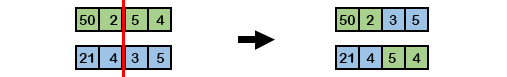
\includegraphics[width=0.9\textwidth]{crossGA.jpg}%
	\vspace{-0.1 cm}
	\captionof{figure}{Croisement de deux solutions.}\label{gacroisement}%
\end{center}


\subsubsection{Mutation}
Une mutation est le remplacement d'un ou plusieurs paramètres de notre solution par une valeur aléatoire, toujours en respectant les contraintes d'intervalle de chaque paramètre cité dans le tableau \ref{ContrGA}. On choisit de faire une seule mutation aléatoire explicitée dans la figure \ref{gamutation} suivante:
\begin{center}	  
	\captionsetup{width=1\linewidth}
	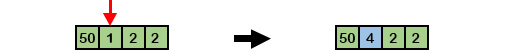
\includegraphics[width=0.9\textwidth]{mutGA.jpg}%
	\vspace{-0.1 cm}
	\captionof{figure}{Mutation d'une solution.}\label{gamutation}%
\end{center}



\subsection{Fonctionnement}
La méta-heuristique GA comporte une population de \textbf{N} individus dont nous essayons d'améliorer les gènes pour obtenir le meilleur individu au fil des générations.
L'organigramme de la figure \ref{ga} décrit ce processus en détail.\\

Tout d'abord, les bornes (inférieurs et supérieurs) de chaque paramètre, pour chaque approche doivent être initialisées, afin que les valeurs générées pour chaque individu soient cohérentes avec l'espace des solutions.
Puis, les \textbf{N} individus de notre population seront générés et évalués un à un selon la fonction objectif décrite plus haut, avant leur insertion dans la population \textbf{P}.
L'auto-paramétrage suit les étapes suivantes :

\subsubsection{Sélection des deux meilleures solutions}
Les deux meilleures solutions de la population \textbf{P} de la  génération \textit{"t$^{i\grave{e}me}$"} sont sélectionnées, soient \textit{"S1"} et \textit{"S2"}.

Ces deux parents sont supprimés de la population après sélection.

\subsubsection{Croisement des deux solutions (parents)}
On effectue lors de cette phase un croisement sur \textit{"S1"} et \textit{"S2"} selon le point de croisement \textbf{pointCroisement}, produisant ainsi deux autres solutions enfants: \textit{"S1$_{fils}$"} et \textit{"S2$_{fils}$"}. 

\subsubsection{Évaluation des solutions fils}
On évalue ensuite les solutions enfants \textit{"S1$_{fils}$"} et \textit{"S2$_{fils}$"} selon la fonction objectif (nombre de cibles trouvées et nombre d'itérations).

\subsubsection{Mutation des solutions fils} 
Les solutions fils subiront un nombre \textbf{nbrMutation} de mutations. Il en résultera deux autres solutions mutantes, qu'on notera : \textit{"S1'$_{fils}$"} et \textit{"S2'$_{fils}$"}. 

\subsubsection{Évaluation des solutions mutantes}
Comme pour les solutions fils, les solutions mutantes seront évaluées selon la fonction objectif.

\subsubsection{Injection des solutions résultantes dans la population}
Une fois les quartes solutions évaluées à savoir : \textit{"S1$_{fils}$"}, \textit{"S2$_{fils}$"}, \textit{"S1'$_{fils}$"} et \textit{"S2'$_{fils}$"}, on les insère dans la population courante.

\subsubsection{Passage à la génération suivante}
Après avoir enrichie la population avec les nouveaux individus, on incrémente  l'indice de génération \textit{"t"}, afin de passer à la génération suivante.

\subsubsection{Critère d'arrêt}
Toutes ces étapes du processus de paramétrage par l'algorithme génétique, seront réitérées jusqu'à ce que le nombre de générations \textbf{MaxGen} soit atteint. 



Pour notre solution finale, nous sélectionnons les cinq meilleures solutions de la population, pour en calculer la moyenne.


\noindent
\begin{center}	  
	\captionsetup{width=1\linewidth}
	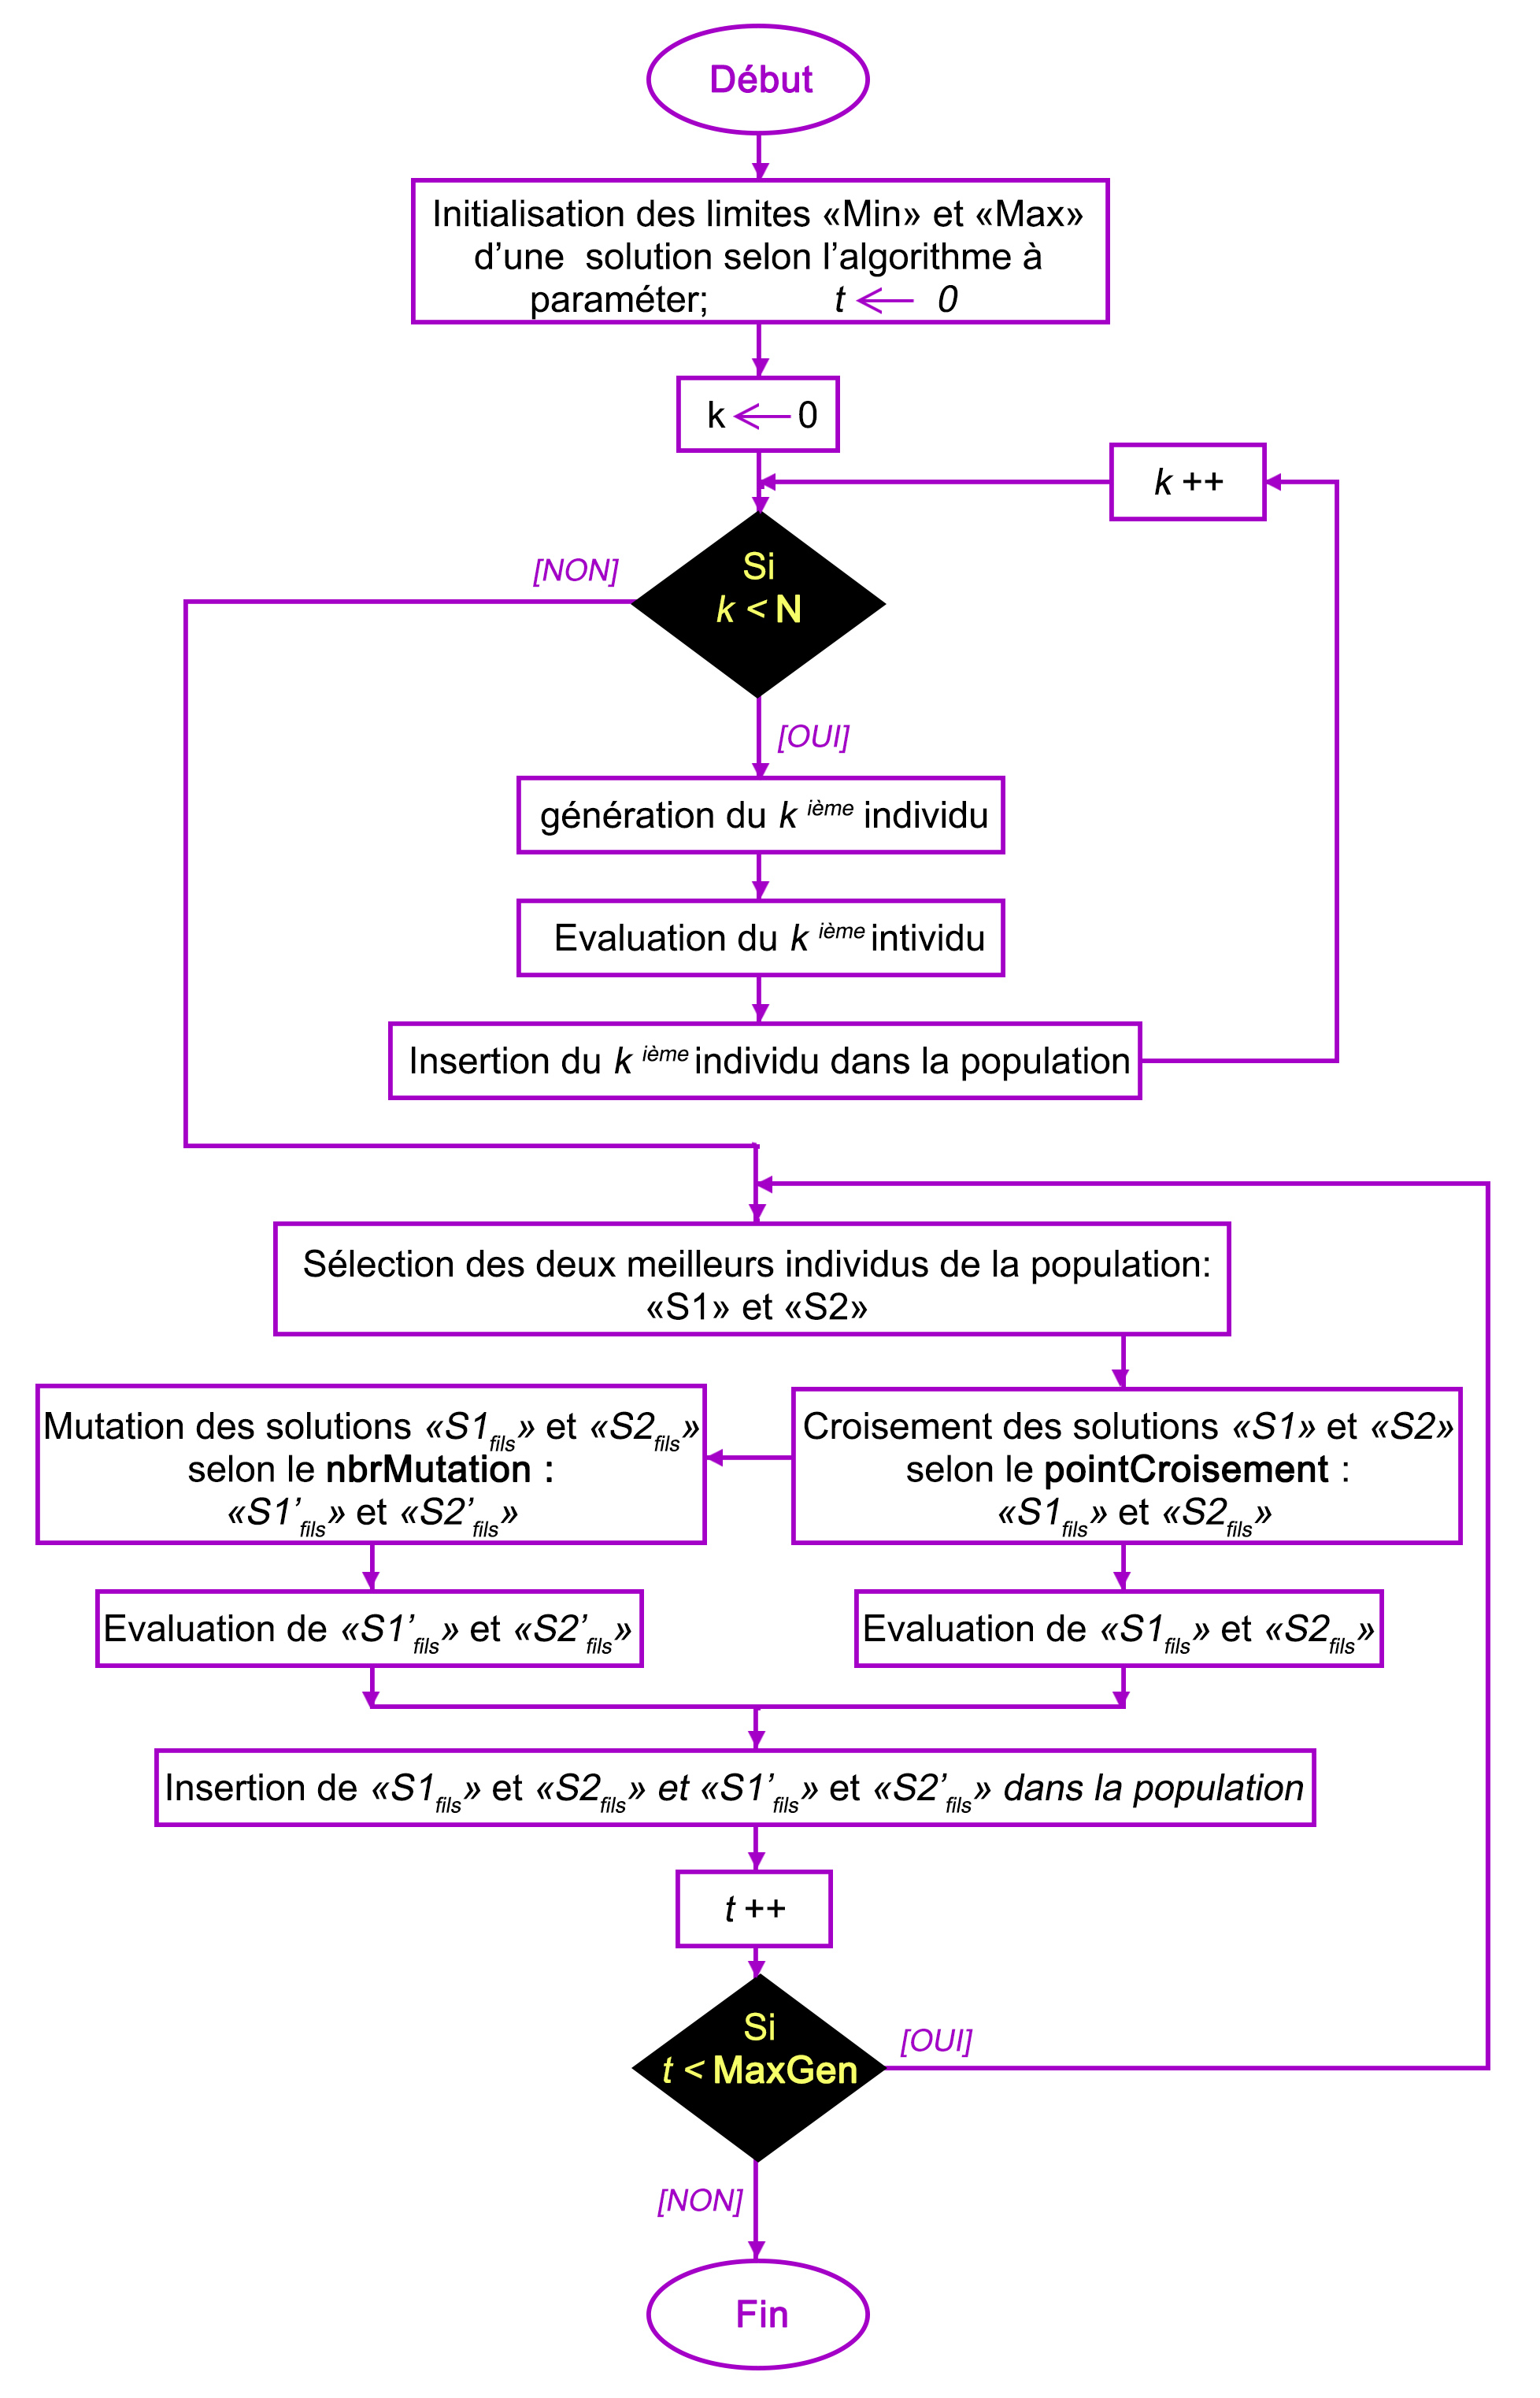
\includegraphics[width=0.79\textwidth]{ga.jpg}%
	\vspace{-0.3 cm}
	\captionof{figure}{Organigramme du mode de fonctionnement de la méthode GA.}\label{ga}%
\end{center}


\section{Conclusion}
Ce chapitre a fait l'objet de la modélisation de tous les aspects de notre problème, c'est à partir de cette modélisation que nous avons choisie une stratégie d'évitement d'obstacles applicable à toutes nos méthodes de résolution basées essaims. Tous les détails relatifs à son fonctionnement y sont présentés. Enfin, nous avons explicité l'usage de l'algorithme Génétique pour le paramétrage automatique.
Ces parties communes à l'ensemble de nos approches de recherche de cibles définies, nous nous attelons à présenter nos approches de recherche de cibles, commençant par BSO dont il est question dans le chapitre suivant.


